\begin{answer}

    \begin{table}[H]
        \centering
        \begin{tabular}{l l}
            \toprule
            \textbf{Dataset} & \textbf{Final $\theta$ (with regularization)} \\
            \midrule
            A & $[-85.22,\;\; 83.00,\;\; 73.40]$ \\
            B & $[-265.60,\;\; 267.25,\;\; 265.40]$ \\
            \bottomrule
        \end{tabular}
        \caption{Final model parameters ($\theta$) after training with regularization}
    \end{table}

Dataset B seems to have smaller parameters, having decreased for each component, being now in the range of Dataset A's parameters. The model's decision boundary has shifted a bit lower, and now isn't perfectly classifying the data anymore; the rate of false positives has increased.

$\rightarrow$ Bias has increased, while the variance decreased.

Dataset A seems to have a similar phenomenon where the decision boundary is not as close anymore to the ``boundary zone'' where points of different label are frequent, but shifts towards the red points, increasing false negatives. The flexibility of the model seems to decrease while the bias increases.

What we observe with A \& B would be desirable if we tried to train a model that should generalize across different datasets, which in themselves have considerable noise. If we assume that the data we are training on is not noisy, we could easily make the model a bit more flexible and fit the data a bit more for better performance.

Regularization also provides benefits besides that as well, such as sparsity, which leads to higher understandability, as it forces the model implicitly to prioritize \emph{relevant} features and keeps weights in a stable range where numerical errors are also reduced.


\begin{figure}[H]
    \centering
    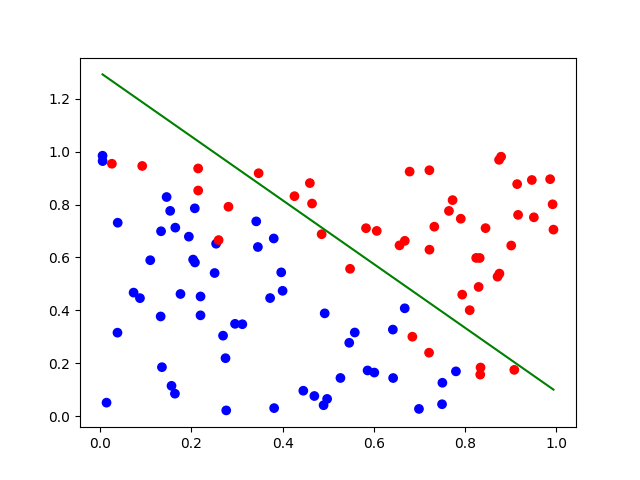
\includegraphics[width=0.6\textwidth]{src/logreg_stability/logreg_pred_a_reg.png}
    \caption{LR decision boundary for dataset A (Regularized)}
\end{figure}


\begin{figure}[H]
    \centering
    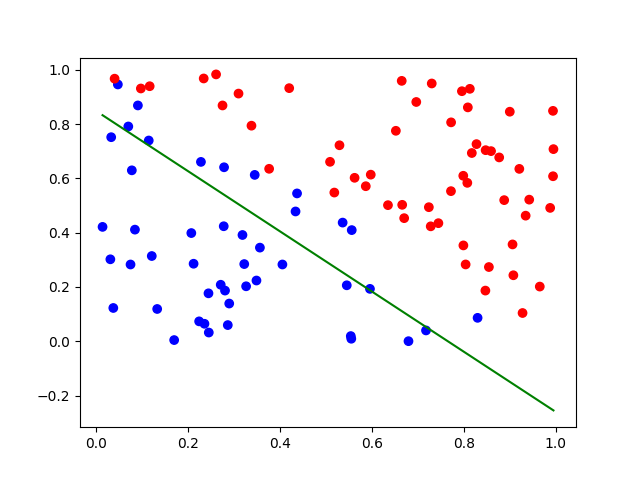
\includegraphics[width=0.6\textwidth]{src/logreg_stability/logreg_pred_b_reg.png}
    \caption{LR decision boundary for dataset B (Regularized)}
\end{figure}

\end{answer}
